\documentclass[report, 12pt]{uftreport}

\title{Máquina de Turing de Duas Fitas para Operações Lógicas Bit a Bit}
\foreigntitle{Two-Tape Turing Machine for Bitwise Logical Operations}

\author{Pedro Lucas}{Moreira Pinto}
\author{Pedro Ryan}{Oliveira de Almeida}
\department{CC}
\class{Teoria da Computação -- 2026.2}

\date{01}{10}{2026}

\keyword{Máquina de Turing}
\keyword{JFLAP}
\keyword{Operações lógicas}
\keyword{Múltiplas fitas}

\foreignkeyword{Turing Machine}
\foreignkeyword{JFLAP}
\foreignkeyword{Logical operations}
\foreignkeyword{Multi-tape}

\lstset{
  literate=
    {á}{{\'a}}1 {à}{{\`a}}1 {ã}{{\~a}}1 {â}{{\^a}}1
    {é}{{\'e}}1 {ê}{{\^e}}1 {í}{{\'i}}1 {ó}{{\'o}}1
    {õ}{{\~o}}1 {ú}{{\'u}}1 {ç}{{\c{c}}}1
    {□}{{$\square$}}1 {→}{{$\rightarrow$}}1 {δ}{{$\delta$}}1
    {│}{{$\vert$}}1 {━}{{-}}1 {┝}{{$\vdash$}}1 {─}{{-}}1,
}

\lstdefinestyle{python}{
  language=Python,
  basicstyle=\ttfamily\scriptsize,
  keywordstyle=\color{uftazul}\bfseries,
  stringstyle=\color{uftverde},
  numbers=left,
  tabsize=4,
  columns=fullflexible,
  keepspaces=true,
}
\lstdefinestyle{terminal}{
  basicstyle=\ttfamily\footnotesize,
  numbers=none,
  frame=single,
  columns=fullflexible,
  keepspaces=true,
}

\renewcommand{\lstlistingname}{Código}
\renewcommand{\lstlistlistingname}{Lista de códigos}

\begin{document}

\frontmatter
\maketitle
\makefrontpage

\tableofcontents
\listoffigures
\listoftables
\lstlistoflistings

\mainmatter
\ChapterStart{first}{Introdução}

\section{Objetivo}

Construir uma Maquina de Turing que, dada uma entrada na forma
\[
  \mathit{op}\; w_1 \,\#\, w_2, \qquad w_1, w_2 \in \{0,1\}^n,
\]
calcule $w_1 \;\mathit{op}\; w_2$ bit a bit, deixando o resultado na fita~2,
onde $\mathit{op}$ é uma das operações da Tabela~\ref{tab:operadores}.

\begin{table}[htbp]
  \centering
  \caption{Símbolos de operação aceitos}
  \label{tab:operadores}
  \begin{tabular}{ccl}
    \toprule
    \textbf{Símbolo} & \textbf{Operação} & \textbf{Ramo de estados} \\
    \midrule
    \texttt{A} & \textsc{and} ($\land$)    & $q_1 \to q_4 \to q_5$ \\
    \texttt{X} & \textsc{xor} ($\oplus$)   & $q_2 \to q_7 \to q_8$ \\
    \texttt{O} & \textsc{or}  ($\lor$)     & $q_3 \to q_9 \to q_{10}$ \\
    \bottomrule
  \end{tabular}
\end{table}

\chapter{Desenvolvimento}

\section{Diagrama de estados}

A Figura~\ref{fig:diagrama} mostra o diagrama construído no JFLAP. A máquina
possui três ramos paralelos e simétricos, um para cada operação, que
convergem no estado de aceitação $q_6$.

\begin{figure}[htbp]
  \centering
  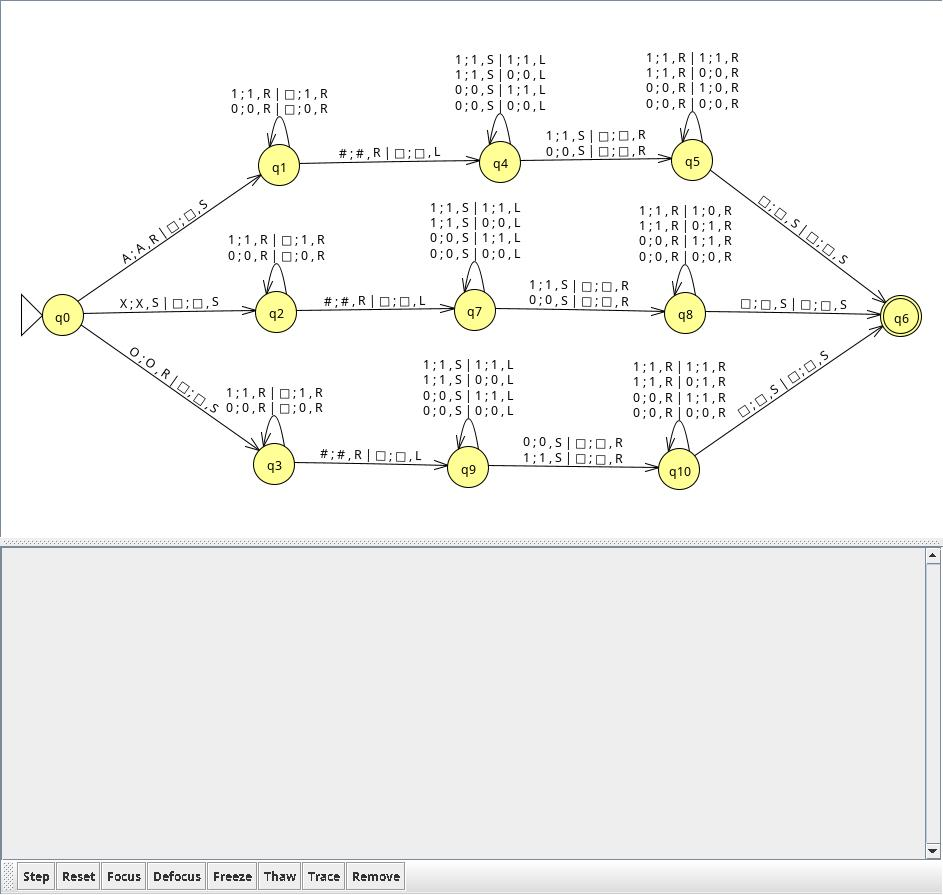
\includegraphics[width=\textwidth,trim=0 360 0 0,clip]{figuras/trabalho1.jpg}
  \caption{Diagrama de estados da Maquina de Turing no JFLAP}
  \label{fig:diagrama}
\end{figure}

\section{Funcionamento}

Inicialmente a fita~1 contém a entrada e a fita~2 está vazia. O
processamento ocorre em quatro fases.

\subsection{Fase 1 --- Seleção da operação ($q_0$)}

Em $q_0$ a máquina lê o primeiro símbolo da fita~1, que identifica a
operação, avança a cabeça da fita~1 e desvia para o ramo correspondente:
\texttt{A} $\to q_1$, \texttt{X} $\to q_2$, \texttt{O} $\to q_3$.

\subsection{Fase 2 --- Cópia do primeiro operando ($q_1$, $q_2$, $q_3$)}

Cada bit de $w_1$ lido na fita~1 é escrito na fita~2, e ambas as cabeças
avançam para a direita (\texttt{0;0,R | $\square$;0,R} e
\texttt{1;1,R | $\square$;1,R}). Ao encontrar \texttt{\#}, a cabeça da
fita~1 passa ao primeiro bit de $w_2$ e a da fita~2 recua para o último bit
copiado, indo para $q_4$, $q_7$ ou $q_9$.

\subsection{Fase 3 --- Retorno da fita 2 ($q_4$, $q_7$, $q_9$)}

A cabeça da fita~1 permanece parada sobre o primeiro bit de $w_2$ enquanto a
da fita~2 se desloca para a esquerda sobre os bits de $w_1$. Ao alcançar o
branco à esquerda de $w_1$, ela avança uma posição e a máquina passa para
$q_5$, $q_8$ ou $q_{10}$, com as duas cabeças alinhadas no bit mais
significativo de cada operando.

\subsection{Fase 4 --- Cálculo bit a bit ($q_5$, $q_8$, $q_{10}$)}

Ambas as cabeças avançam juntas. A cada passo, o bit $b_1$ da fita~1 (de
$w_2$) e o bit $b_2$ da fita~2 (de $w_1$) são combinados e o resultado
sobrescreve $b_2$ na fita~2. A Tabela~\ref{tab:verdade} resume as
transições de laço de cada estado. Quando as duas fitas leem $\square$, a
máquina transita para $q_6$ e aceita.

\begin{table}[htbp]
  \centering
  \caption{Valor escrito na fita 2 em cada estado de cálculo}
  \label{tab:verdade}
  \begin{tabular}{cccccc}
    \toprule
    \textbf{Fita 1} & \textbf{Fita 2} & & $q_5$ (\textsc{and})
      & $q_8$ (\textsc{xor}) & $q_{10}$ (\textsc{or}) \\
    \midrule
    0 & 0 & & 0 & 0 & 0 \\
    0 & 1 & & 0 & 1 & 1 \\
    1 & 0 & & 0 & 1 & 1 \\
    1 & 1 & & 1 & 0 & 1 \\
    \bottomrule
  \end{tabular}
\end{table}

\section{Exemplos de execução}

A Tabela~\ref{tab:exemplos} apresenta entradas testadas e o conteúdo final
da fita~2.

\begin{table}[htbp]
  \centering
  \caption{Exemplos de entradas e resultados}
  \label{tab:exemplos}
  \begin{tabular}{lcc}
    \toprule
    \textbf{Entrada (fita 1)} & \textbf{Resultado (fita 2)} & \textbf{Situação} \\
    \midrule
    \texttt{A110\#101}    & \texttt{100}  & aceita \\
    \texttt{X110\#101}    & \texttt{011}  & aceita \\
    \texttt{O110\#101}    & \texttt{111}  & aceita \\
    \texttt{O0011\#0101}  & \texttt{0111} & aceita \\
    \texttt{A1\#0}        & \texttt{0}    & aceita \\
    \bottomrule
  \end{tabular}
\end{table}

\subsection{Rastreamento de \texttt{A110\#101}}

\begin{enumerate}
  \item $q_0$: lê \texttt{A}, vai para $q_1$.
  \item $q_1$: copia \texttt{110} para a fita~2; ao ler \texttt{\#} vai para $q_4$.
  \item $q_4$: recua a fita~2 até o início de \texttt{110}; vai para $q_5$.
  \item $q_5$: calcula $1\land1=1$, $1\land0=0$, $0\land1=0$, deixando
        \texttt{100} na fita~2.
  \item Lê $\square$ nas duas fitas e aceita em $q_6$.
\end{enumerate}

\section{Limitações}

\begin{itemize}
  \item Os operandos devem ter o mesmo comprimento. Se $w_2$ for mais longo,
        a fita~2 lê $\square$ durante o cálculo e a máquina para sem aceitar;
        se for mais curto, a máquina aceita deixando bits de $w_1$ não
        processados na fita~2.
  \item Não há validação de símbolos inesperados; nesses casos a máquina
        simplesmente para em estado não final.
\end{itemize}


\chapter{Código-fonte}


Para executar:

\begin{lstlisting}[style=terminal]
python3 main.py             # tabela-resumo dos exemplos
python3 main.py A110#101    # execução passo a passo
\end{lstlisting}

\section{Módulo \texttt{fita.py}: representação das fitas}

A classe \texttt{Fita} armazena os símbolos em um dicionário indexado pela posição, o que permite que a fita seja infinita nos dois sentidos. O atributo \texttt{cabeca} guarda explicitamente a posição da cabeça de leitura e escrita.

\begin{lstlisting}[style=python, caption={Módulo \texttt{fita.py}: representação das fitas}, label={lst:fita}]
BRANCO = "□"
PASSO_DA_CABECA = {"R": +1, "L": -1, "S": 0}

class Fita:

    def __init__(self, conteudo=""):
        self.simbolos = dict(enumerate(conteudo))
        self.cabeca = 0

    def ler(self):
        return self.simbolos.get(self.cabeca, BRANCO)

    def escrever(self, simbolo):
        self.simbolos[self.cabeca] = simbolo

    def mover(self, direcao):
        self.cabeca += PASSO_DA_CABECA[direcao]

    def conteudo(self):
        return "".join(s for _, s in sorted(self.simbolos.items()) if s != BRANCO)

    def desenhar(self, inicio, fim):
        celulas = []
        for pos in range(inicio, fim + 1):
            s = self.simbolos.get(pos, BRANCO)
            celulas.append(f"[{s}]" if pos == self.cabeca else f" {s} ")
        return "".join(celulas)
\end{lstlisting}

\section{Importações e constantes}

Definição do símbolo branco ($\square$), do estado inicial e do conjunto de estados finais.

\begin{lstlisting}[style=python, caption={Importações e constantes}, label={lst:const}]
import sys
from collections import namedtuple
from fita import Fita
from printout import mostrar_passo_a_passo, mostrar_resumo
BRANCO = "□"
ESTADO_INICIAL = "q0"
ESTADOS_FINAIS = {"q6"}
\end{lstlisting}

\section{Função de transição $\delta$}

Cada regra é uma \texttt{Transicao} indexada pela tupla (estado, símbolo lido na fita~1, símbolo lido na fita~2), correspondendo diretamente às transições do diagrama da Figura~\ref{fig:diagrama}.

\begin{lstlisting}[style=python, caption={Função de transição $\delta$}, label={lst:delta}]
Transicao = namedtuple("Transicao", "proximo escreve1 escreve2 move1 move2")

DELTA = {
    ("q0", "A", BRANCO): Transicao("q1", "A", BRANCO, "R", "S"),
    ("q0", "X", BRANCO): Transicao("q2", "X", BRANCO, "R", "S"),
    ("q0", "O", BRANCO): Transicao("q3", "O", BRANCO, "R", "S"),

    ("q1", "0", BRANCO): Transicao("q1", "0", "0", "R", "R"),
    ("q1", "1", BRANCO): Transicao("q1", "1", "1", "R", "R"),
    ("q1", "#", BRANCO): Transicao("q4", "#", BRANCO, "R", "L"),

    ("q2", "0", BRANCO): Transicao("q2", "0", "0", "R", "R"),
    ("q2", "1", BRANCO): Transicao("q2", "1", "1", "R", "R"),
    ("q2", "#", BRANCO): Transicao("q7", "#", BRANCO, "R", "L"),

    ("q3", "0", BRANCO): Transicao("q3", "0", "0", "R", "R"),
    ("q3", "1", BRANCO): Transicao("q3", "1", "1", "R", "R"),
    ("q3", "#", BRANCO): Transicao("q9", "#", BRANCO, "R", "L"),

    ("q4", "0", "0"):    Transicao("q4", "0", "0", "S", "L"),
    ("q4", "0", "1"):    Transicao("q4", "0", "1", "S", "L"),
    ("q4", "1", "0"):    Transicao("q4", "1", "0", "S", "L"),
    ("q4", "1", "1"):    Transicao("q4", "1", "1", "S", "L"),
    ("q4", "0", BRANCO): Transicao("q5", "0", BRANCO, "S", "R"),
    ("q4", "1", BRANCO): Transicao("q5", "1", BRANCO, "S", "R"),

    ("q7", "0", "0"):    Transicao("q7", "0", "0", "S", "L"),
    ("q7", "0", "1"):    Transicao("q7", "0", "1", "S", "L"),
    ("q7", "1", "0"):    Transicao("q7", "1", "0", "S", "L"),
    ("q7", "1", "1"):    Transicao("q7", "1", "1", "S", "L"),
    ("q7", "0", BRANCO): Transicao("q8", "0", BRANCO, "S", "R"),
    ("q7", "1", BRANCO): Transicao("q8", "1", BRANCO, "S", "R"),

    ("q9", "0", "0"):    Transicao("q9", "0", "0", "S", "L"),
    ("q9", "0", "1"):    Transicao("q9", "0", "1", "S", "L"),
    ("q9", "1", "0"):    Transicao("q9", "1", "0", "S", "L"),
    ("q9", "1", "1"):    Transicao("q9", "1", "1", "S", "L"),
    ("q9", "0", BRANCO): Transicao("q10", "0", BRANCO, "S", "R"),
    ("q9", "1", BRANCO): Transicao("q10", "1", BRANCO, "S", "R"),

    ("q5", "0", "0"):         Transicao("q5", "0", "0", "R", "R"),
    ("q5", "0", "1"):         Transicao("q5", "0", "0", "R", "R"),
    ("q5", "1", "0"):         Transicao("q5", "1", "0", "R", "R"),
    ("q5", "1", "1"):         Transicao("q5", "1", "1", "R", "R"),
    ("q5", BRANCO, BRANCO):   Transicao("q6", BRANCO, BRANCO, "S", "S"),

    ("q8", "0", "0"):         Transicao("q8", "0", "0", "R", "R"),
    ("q8", "0", "1"):         Transicao("q8", "0", "1", "R", "R"),
    ("q8", "1", "0"):         Transicao("q8", "1", "1", "R", "R"),
    ("q8", "1", "1"):         Transicao("q8", "1", "0", "R", "R"),
    ("q8", BRANCO, BRANCO):   Transicao("q6", BRANCO, BRANCO, "S", "S"),

    ("q10", "0", "0"):        Transicao("q10", "0", "0", "R", "R"),
    ("q10", "0", "1"):        Transicao("q10", "0", "1", "R", "R"),
    ("q10", "1", "0"):        Transicao("q10", "1", "1", "R", "R"),
    ("q10", "1", "1"):        Transicao("q10", "1", "1", "R", "R"),
    ("q10", BRANCO, BRANCO):  Transicao("q6", BRANCO, BRANCO, "S", "S"),
}
\end{lstlisting}

\section{Descrição das fases}

Tabela usada apenas na exibição, associando cada estado à fase do algoritmo.

\begin{lstlisting}[style=python, caption={Descrição das fases}, label={lst:fase}]
FASE = {
    "q0": "Fase 1: lê o operador",
    "q1": "Fase 2: copia w1 para a fita 2 (AND)",
    "q2": "Fase 2: copia w1 para a fita 2 (XOR)",
    "q3": "Fase 2: copia w1 para a fita 2 (OR)",
    "q4": "Fase 3: volta a cabeça da fita 2 ao início",
    "q7": "Fase 3: volta a cabeça da fita 2 ao início",
    "q9": "Fase 3: volta a cabeça da fita 2 ao início",
    "q5": "Fase 4: calcula w1 AND w2",
    "q8": "Fase 4: calcula w1 XOR w2",
    "q10": "Fase 4: calcula w1 OR w2",
    "q6": "Fim: aceita",
}
PASSO_DA_CABECA = {"R": +1, "L": -1, "S": 0}
\end{lstlisting}

\section{Classe \texttt{MaquinaTuring}}

A máquina mantém explicitamente as duas fitas, o estado atual e a função $\delta$. O método \texttt{executar} aplica transições até alcançar um estado final ou não haver regra definida.

\begin{lstlisting}[style=python, caption={Classe \texttt{MaquinaTuring}}, label={lst:mt}]
class MaquinaTuring:
    def __init__(self, entrada, delta=DELTA):
        self.fita1 = Fita(entrada)
        self.fita2 = Fita()
        self.estado = ESTADO_INICIAL
        self.delta = delta
        self.passos = 0

    def transicao_atual(self):
        return self.delta.get((self.estado, self.fita1.ler(), self.fita2.ler()))

    def passo(self, regra):
        self.fita1.escrever(regra.escreve1)
        self.fita2.escrever(regra.escreve2)
        self.fita1.mover(regra.move1)
        self.fita2.mover(regra.move2)
        self.estado = regra.proximo
        self.passos += 1

    def executar(self, ao_passar=None, limite=10_000):
        while self.estado not in ESTADOS_FINAIS:
            regra = self.transicao_atual()
            if regra is None or self.passos >= limite:
                return False
            lido = (self.fita1.ler(), self.fita2.ler())
            anterior = self.estado
            self.passo(regra)
            if ao_passar:
                ao_passar(self, anterior, lido, regra)
        return True
\end{lstlisting}

\section{Exibição da execução}

Funções responsáveis pela saída: o rastreamento passo a passo, com a troca de estado, a regra aplicada e o conteúdo das fitas, e a tabela-resumo.

\begin{lstlisting}[style=python, caption={Exibição da execução}, label={lst:print}]
def mostrar_passo_a_passo(entrada):
    mt = MaquinaTuring(entrada)
    inicio, fim = -1, len(entrada)
    largura = 3 * (fim - inicio + 1)

    def linha(n, transicao, regra, mt):
        f1 = mt.fita1.desenhar(inicio, fim)
        f2 = mt.fita2.desenhar(inicio, fim)
        print(f"{n:>5} │ {transicao:<11} │ {regra:<21} │ {f1} │ {f2}")

    def ao_passar(mt, anterior, lido, r):
        if FASE[mt.estado] != FASE[anterior]:
            print(f"      ┝━ {FASE[mt.estado]}")
        regra = f"({lido[0]},{lido[1]}) → ({r.escreve1},{r.escreve2},{r.move1},{r.move2})"
        linha(mt.passos, f"{anterior} → {mt.estado}", regra, mt)

    print(f"\nEntrada: {entrada}\n")
    print(f"{'passo':>5} │ {'estado':<11} │ {'lê → escreve, move':<21} │ "
          f"{'fita 1':^{largura}} │ {'fita 2':^{largura}}")
    print("─" * (48 + 2 * largura))
    print(f"      ┝━ {FASE[mt.estado]}")
    linha(0, mt.estado, "configuração inicial", mt)

    aceitou = mt.executar(ao_passar)

    print()
    if aceitou:
        print(f"ACEITA em {mt.passos} passos. Resultado (fita 2): {mt.fita2.conteudo()}")
    else:
        print(f"REJEITA: sem transição em {mt.estado} lendo "
              f"({mt.fita1.ler()}, {mt.fita2.ler()}).")

def mostrar_resumo(entradas):
    print(f"{'entrada':<12} {'resultado':<10} {'situação':<9} passos")
    print("─" * 40)
    for entrada in entradas:
        mt = MaquinaTuring(entrada)
        situacao = "aceita" if mt.executar() else "rejeita"
        print(f"{entrada:<12} {mt.fita2.conteudo():<10} {situacao:<9} {mt.passos}")
\end{lstlisting}

\section{Ponto de entrada}

Sem argumentos, executa os exemplos da Tabela~\ref{tab:exemplos}; com argumentos, mostra o passo a passo de cada entrada.

\begin{lstlisting}[style=python, caption={Ponto de entrada}, label={lst:main}]
if __name__ == "__main__":
    if len(sys.argv) > 1:
        for entrada in sys.argv[1:]:
            mostrar_passo_a_passo(entrada)
    else:
        mostrar_resumo(["A110#110", "A110#101", "X110#101",
                        "O110#101", "O0011#0101", "A1#0"])
        print("\nPasso a passo: python3 main.py A110#101")
\end{lstlisting}

\section{Exemplo de saída}

A Figura~\ref{fig:saida} mostra a execução passo a passo da entrada
\texttt{A110\#101}. Cada linha indica a troca de estado, a regra de $\delta$
aplicada e o conteúdo das duas fitas, com a posição de cada cabeça entre
colchetes. Ao final, a fita~2 contém \texttt{100}, resultado de
$110 \land 101$.

\begin{figure}[htbp]
  \centering
  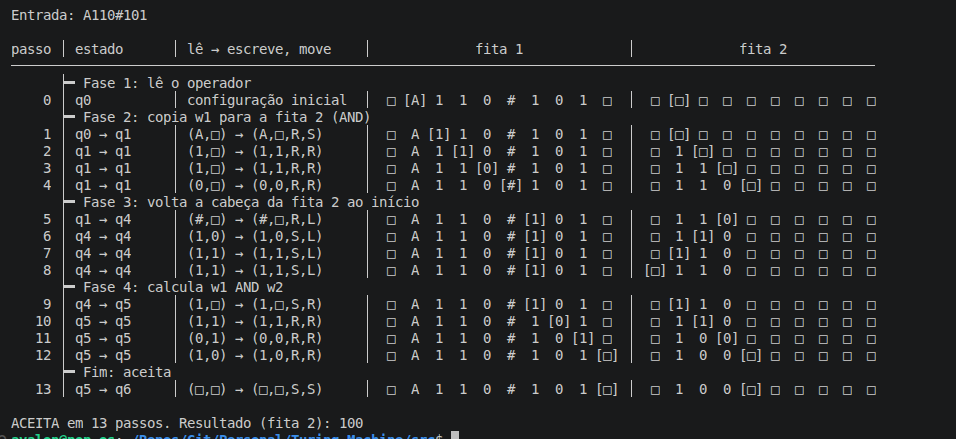
\includegraphics[width=\textwidth]{figuras/image.png}
  \caption{Saída do simulador para a entrada \texttt{A110\#101}}
  \label{fig:saida}
\end{figure}

\chapter{Conclusão}

A Maquina de Turing de duas fitas desenvolvida computa corretamente as operações
\textsc{and}, \textsc{or} e \textsc{xor} entre números binários de mesmo
tamanho. O uso de uma segunda fita permitiu armazenar o primeiro operando e
reaproveitá-lo como área de resultado, evitando idas e vindas na fita de
entrada e mantendo o número de estados pequeno (11 estados). A estrutura em
ramos paralelos também facilita a inclusão de novas operações, bastando
adicionar um novo ramo com a tabela-verdade desejada.

\backmatter


\end{document}
